%\section{Introduction}
%
In this Chapter, the adopted methodologies to perform formal verification and optimal sizing of stand-alone solar PV systems using formal methods, more specifically model checking, will be detailed. Diagrams, flowcharts, and algorithms support and explain the solutions.

Besides that, all the assumptions and premises adopted are presented. Both support the results/conclusions, with direct impact on it. Usually, a premise is an unquestionable fact, however assumptions can be questionable. Unlike the premise, assumptions are not explicitly stated and need to be deciphered. With that in mind, a detailed explanation of assumptions is performed for all over this Chapter.

It is important to emphasize that the whole explanation about the theoretical basis of the two subjects discussed here are present in the previous chapter. In addition, the author suggests that previous reading be done to facilitate understanding.

\section{Automated Verification of Solar PV Systems}

Fig.~\ref{fig:validation} illustrates how a stand-alone solar PV project can be validated, passing through the traditional techniques, as manual, simulation, testing, and including the proposed automatic verification that is detailed in this Section. 

Note that, in one hand, the input information is the same for all the techniques, with the difference that in automated validation it is possible to define the bound $k$ to restrict the space-design search. Among the inputs it is possible to list: location weather data (temperature, solar irradiance, and solar insolation); system sizing information regarding specifications and configuration of PV panels, charge controller, inverter, batteries, DC bus  voltage; and requirements (battery autonomy, electric load demand, electric peak power demand, energy consumption, load curve, and AC voltage).

However, in the other hand, the outputs are not equal, as the design-space coverage and the information presented as result. Regarding the design-space, it was shown in  chapter \nameref{chap:background} that the most complete coverage is performed by automated verification, event using the bound $k$ to restrict the search, because is not necessary to unbound completely the system in order to found a design flaw. Moreover, testing and simulation depends on the test vector used as input to evaluate the system.

About the results presented by the methods, a project validation done 'by hand' is just a piece of paper produced; simulation software produce fail, success information and can additionally to present the optimized design if the evaluated has some flaw, with graphics and reports; testing (using laboratory or field) is done using measurement equipment and/or data from monitoring systems. Automated verification, proposed at this Thesis, presents fail, success information as well, however the output is not graphical (as will be shown in the  \autoref{chap:automatedverification}), summarized by reports with details about the variables and states of the project that causes a project flaw (in the case where is detected a design fail).

\begin{figure}[h]
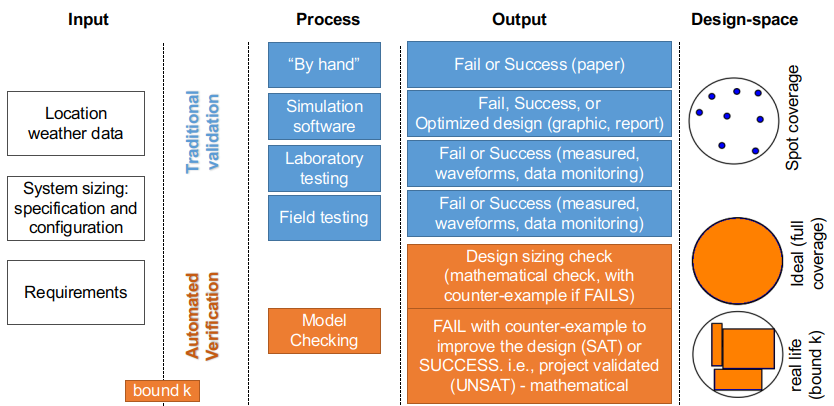
\includegraphics[width=1.0\textwidth]{PVprojectvalidation2}
\centering
\caption{Comparative of project validation methods}
\label{fig:validation}
\end{figure}

Starting at his point, it will be showed how is done the proposed automated verification of stand-alone solar PV systems. 

The process begins with the conversion of the real PV system into a model. The Fig. \ref{fig:systemverif4} shows how a real solar PV system is equivalent and converted to a model in order to be verified by a model checking. 

This illustration is a adaption from the general process of real system conversion depicted in Fig.~\ref{fig:systemverif}, detailing the inputs, outputs, and requirements of a real solar PV system. 

Worth to mention that the model checking process is the same independently of the system that is validated, and the important is to chose a accurate model, to define the requirements/constraints, and to get correct information from the system components, in order to get sound and effective validation,

\begin{figure}[h]
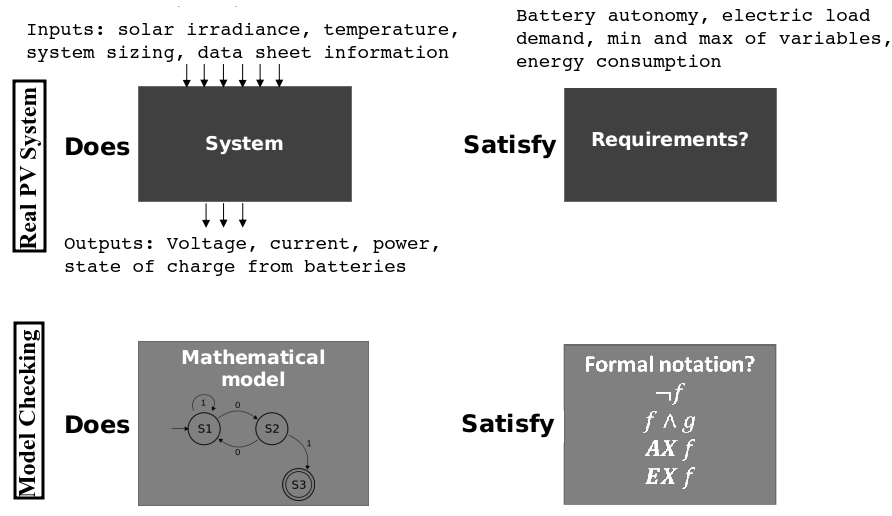
\includegraphics[width=0.8\textwidth]{systemverif4}
\centering
\caption{From real solar PV system verification to model checking. Source: adapted from \cite{Clarke2008}.}
\label{fig:systemverif4}
\end{figure}

Moreover, the proposed flowchart of the automated verification method is illustrated in Fig.~\ref{fig:flowchartgeneral}. Those three steps are the high level description of how the automated verification, applied to solar PV systems, works.

\begin{figure}[h]
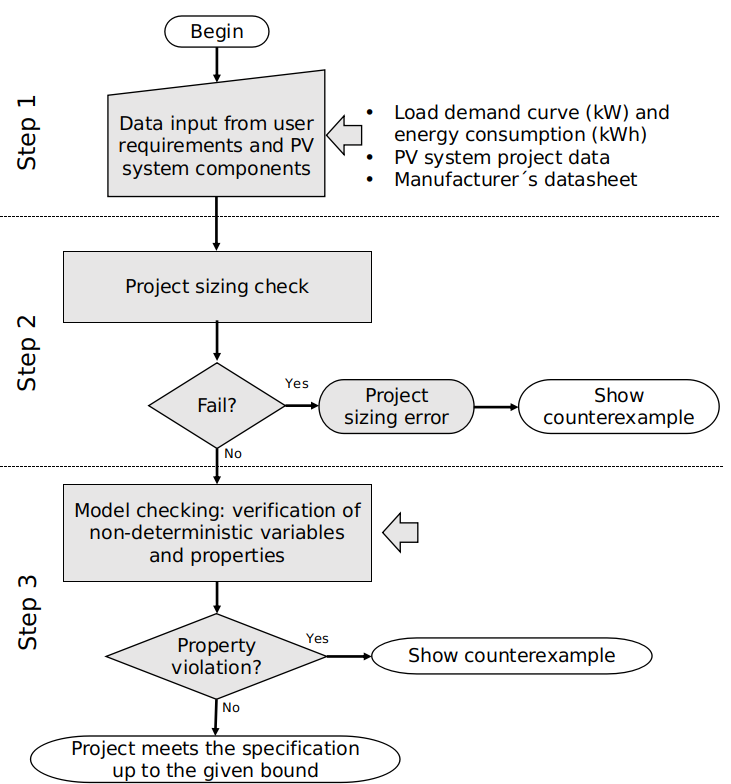
\includegraphics[width=0.6\textwidth]{flowchart_verification5.png}
\centering
\caption{Flowchart of the proposed automated verification of PV systems.}
\label{fig:flowchartgeneral}
\end{figure}

In \textbf{Step 1}, the PV input data %(e.g., load power demand and load energy consumption) 
and the formulae to check the sizing project, the mathematical model, the limits of the weather non-deterministic variables, are all written as an ANSI-C code~\cite{ANSI2018}. 

\textbf{Assumption:} All the PV system model, user requirements, assumptions, and technical information from the PV system equipment is written as an ANSI-C code.

In \textbf{Step 2}, the sizing check of the PV system takes place: it will indicate if there is an error of sizing before to perform the automated verification of the system. This stage ensures that the system meets the standard project steps related to critical period method of sizing~\cite{Pinho}. 

\textbf{Assumption:} before the automated verification, who performs the verification of the intended system behavior, is performed the sizing checking of the system. Moreover, if there is some error, the process stops, showing where is the sizing error.

\textbf{Assumption:} Sizing check is performed using critical period criteria.

In \textbf{Step 3}, weather variables (e.g., solar irradiance and ambient temperature) will be systematically explored by our verification engine based on maximum and minimum values from the site, where the PV system will be deployed. 
%As a consequence, all the formulae of the employed mathematical models will also be updated. 
In addition, depending on one of the desired properties of the system such as battery autonomy, energy availability, or even system power supply, our verification engine is able to indicate a failure if those properties are not met; in this particular case, it provides a diagnostic counterexample that shows in which conditions the property violation occurred. 
%; as the  state of charge of the batteries, load demand of power and the load consumption of energy if defined by the code
% (as reliability, performance, or safety)

%
%\textcolor{red}{In the following paragraph you should related the output of our verification engine with the description of the BMC SAT or UNSAR given above. For example, what does a failure mean? is it SAT?}
In a nutshell, the model checker will process the ANSI-C code with constraints ($C$) and properties ($P$) from the PV system, and the tool will automatically verify if the PV system requirements are met. If it returns a failure (i.e., SAT), then the tool provides a counterexample, i.e., a sequence of states that leads to the property violation; this information can be used as a feedback to improve the PV system design. However, if the verification succeeds (i.e., UNSAT), there is no failure up to the bound $k$; therefore, the PV system will present its intended behavior up to the bound $k$.

\textbf{Assumption:} Use of bound $k$ to restrict the design-space and improve performance.

%, i.e., our verification engine does not give any guarantee that there is no error in bound $k+1$ unless some induction method is employed~\cite{DBLP:journals/sttt/GadelhaIC17}.
%
%
%---------------------------------------------------------------------
% \subsection{The case studies and the Algorithm}
%---------------------------------------------------------------------
%
% 
%and as backup at night 
%
%The 700 W system: 3 x 325 W PV panels connected in series, controller of 150 V/35 A with a DC-bus of 24 V, 4 x 220 Ah batteries (2 in series and 2 in parallel arrangement), and inverter of 700 W. 
%
%And the 1,200 W PV system: 4 x 325 W connected in series PV panels, with controller of 150 V/35 A  in a DC-bus of 48 V, 4 batteries of 120 Ah connected in series, and a 1,200 W inverter.
%
%As demonstrated at this work, the performance of the system is highly dependent of solar irradiance and temperature, that are specific of the deployed local (latitude and longitude). 

Algorithm~\ref{alg:verification-algorithm} describes the equivalent pseudo-code. %Line 1 indicates a function call that performs the size checking of the each component of the PV system. %: using Equations \eqref{eq:NTPmin}, \eqref{eq:NTP}, \eqref{eq:NPSmin}, \eqref{eq:NPS}, \eqref{eq:NPP}, and \eqref{eq:NPPmin} to verify the PV panel; using \eqref{eq:Cbank}, \eqref{eq:Nbtotal}, and \eqref{eq:batcheck} to verify the batteries; using \eqref{eq:vcvsystem}, \eqref{eq:icmin}, and \eqref{eq:icicmin} to verify the charge controller; and using \eqref{eq:vindc}, \eqref{eq:voutac}, and \eqref{eq:invcheck} to verify the inverter. 
%The verification is carried out by the \textit{assert} macro from the ANSI-C programming language to encode each equation of sizing check. The argument to the \textit{assert} statement must be \textit{true} if the system specification is met; otherwise, the program aborts and prints a counterexample indicating a property violation. If there is no property violation, then the verification algorithm continues and 
In order to reduce the computational effort of the algorithm,
% caused by the state explosion inherent of the technique, 
every 24 h-day was considered as a time-step of 1 hour, and it was split into two parts: (a) one where it is possible to occur PV generation, during daylight, with a duration in hours depending on each site (but dependent on the sun and weather conditions); and (b) one that includes all the remaining day (without any PV generation), when the batteries are demanded to feed the house.

\textbf{Assumption:} day is divided in two parts (when there is and there is not PV generation, based in historical data from the location). Considering average temperature and solar irradiance (for every hour of the day) and the annual solar insolation (per day).

Lines 1 is devoted to information from the location where the PV system will be/were deployed. We use annual average minimum and maximum, related to temperature ($T$) and solar irradiance ($G$), hour by hour, from~\cite{Temperature}, and ~\cite{Irradiance}.

\textbf{Premise:} The availability of temperature, solar irradiance, and solar insolation data from the location where the solar PV system will be used.

Line 2 represents all the information that comes from the PV sizing and from the equipment manufacturers data: specification and data from PV, batteries, inverter and charge controller. This item includes as information from the house's load curve.

\textbf{Premise:} Availability of data sheet from every element of the solar PV system to be validated.

\textbf{Premise:} It is necessary the detailed sized project of the PV system in order to perform the validation (list of equipment and configuration, as voltage, current and how they are connected).

\textbf{Assumption:} Load curve from every house must be estimated or measured. Moreover, the time step is of 1 hour, and it is not considered seasonality, i.e., the load curve is the same for the entire year.

The first automated verification is related to the sizing check (line 3), if an error is found then the algorithm stops. In order to perform the sizing check, the algorithm uses Equations \eqref{eq:NTPmin}, \eqref{eq:NPSmin}, and \eqref{eq:NPPmin} to verify the PV panel; using \eqref{eq:Nbtotal}, and \eqref{eq:batcheck} to verify the batteries; using \eqref{eq:vcvsystem}, \eqref{eq:icmin}, and \eqref{eq:icicmin} to verify the charge controller; and using \eqref{eq:vindc}, \eqref{eq:voutac}, and \eqref{eq:invcheck} to verify the inverter.

Then, if there is not a sizing design flaw, two functions, called at lines 4 and 5, are responsible for discover which hour starts the PV generation and when stops. Those functions get this information from the array inputted to the Algorithm with the solar irradiance values.

The batteries are assumed to be charged, i.e., with SOC of 100\% (line 6).

\textbf{Assumption:} Batteries are considered charged at the beginning of the project validation.

The first for-loop at line 7 controls how many cycles of 24 h will be performed by the Algorithm.  And the for-loop from lines 8 to 11 is responsible to discharge the battery (according the load curve) and verify the state of charge of the battery, hour-by-hour, starting at the first hour of the day after the sun goes down until the next day before the sun goes up (without PV generation). Following, at the next for-loop, from line 12 to 29, is performed the verification where there is solar irradiance and all the PV system works. The Algorithm generates information related to average temperature ($T$) and solar irradiance ($G$), hour-by-hour, using non-deterministic variables from model checker to explore all possible states and the \textit{assume} macro to constrain the non-deterministic values using a given range (lines 15 and 16). 
%and irradiance varies from 0 W/m$^{2}$ to 852 W/m$^{2}$ (with minimum of 274 W/m$^{2}$ during the daytime, when there is sunlight). 
%there is PV generation only between 8:00 h and 16:00 h every day, 
%with zero electric energy generation from 18:00 h to 6:00 h of the next day; and with insignificant generation from 6:00 h to 8:00 h, and from 16:00 h to 18:00 h of the same day. 

After that, the model from PV generator is used in the function call of line 17, to produce the voltage and current considering the states of $G$ and $T$. With respect to every hour considered, the conditional \textit{if-elseif-endif} statements from lines 18, 20, 22, 24 and 26, will imitate the charge controller work as depicted in Table~\ref{table:controller} of Section~\ref{sec:controller}, performing the charge or discharge of batteries according to the value of different variables: if there is PV generation, the updated state of charge from batteries, the house's load and the set-up information of the PV system.

At the end of last for-loop, the state of the batteries is verified again (line 27) and the hour is adjusted to the next loop (line 28).

Nevertheless, if the verification engine does not fail, we can conclude that the PV system does not need further corrections up to the given bound $k$.
%
%\textcolor{red}{this sentence is unclear... After this process is started the battery autonomy verification, from line 31}. \textcolor{red}{this sentence is unclear... Based on the fact that won't be PV generation after a given time of the day, the algorithm will only discharge the batteries until a new charging process (at the next day) to start.} \textcolor{red}{what do you mean by The formal verification is guaranteed?...  The formal verification is guaranteed by  macro to specific variables of the model, according lines 27 and 35.}
% and the non-deterministic variables $G$ and $T$ are considered during the formal verification of the system, otherwise, during the other two periods, there is no PV generation and just the power consumption from the backup batteries. 
%Within this 8h-period, $G$ and $T$ are automated verified with different values every one hour.
%, and change their value every 1 h according with the algorithm created using the technique.
 \begin{algorithm}
 \caption{Model checking algorithm for validation of stand-alone PV systems}
 \begin{algorithmic}[1]
 \begin{scriptsize}
 \renewcommand{\algorithmicrequire}{\textbf{Input:}}
 \renewcommand{\algorithmicensure}{\textbf{Output:}}
  \STATE $declare \, min \, and \, max \, solar \, irradiation[24h], \, and \, temperature[24h]$\\
  \STATE $declare \, case \, studies \, details: \, sizing \, and \, manufacturers \, data $ \\
  \STATE $sizing \_ check()$ \\
  \STATE $startPVgeneration \leftarrow findStartPVgeneration()$ \\
  \STATE $endPVgeneration \leftarrow findEndPVgeneration()$ \\
  \STATE $SOC \leftarrow 100\%$ \\
%  \COMMENT {Starting with the PV generation time}
% \\ 
%\textit{LOOP Process}
 \FOR {$1st \, 24h \, loop$ to $Nth \, 24h \, loop$}
  \FOR {$endPVgeneration+1$ to $startPVgeneration-1$}
	  \STATE $dischargeBattery \, in \, 1h()$ \\
%	  \STATE $autonomyCount \leftarrow autonomyCount+1$ \\
	  \STATE $assert (SOC \geq SOC \_ min)$ \\
%	  \STATE $battery \, autonomy \, verification()$ \\
  \ENDFOR
  \FOR {$startPVgeneration$ to $endPVgeneration$}
    \STATE $G \leftarrow nondet \_ uint(\,)$ \COMMENT {$G$ is non-deterministic variable}
    \STATE $T \leftarrow nondet \_ uint(\,)$ \COMMENT {$T$ is non-deterministic variable}
    \STATE assume ($Gmin \leq G \leq Gmax$) \COMMENT {restricting $G$ values}
    \STATE assume ($Tmin \leq T \leq Tmax$) \COMMENT {restricting $T$ values}
    \STATE $Imax, Vmax \leftarrow PVgenerationMODEL (G,T)$ \\
    \COMMENT {If-then-else sequence to imitate charge controller work}
    \IF {($battery \, is \, empty$) AND ($PV \, is \, generating$)}
      \STATE $chargeBattery \, in \, 1h()$ \COMMENT {PV feed the house}
    \ELSIF {($battery \, is \, empty$) AND NOT($PV \, is \, generating$)}
      \STATE FAIL with assert macro \COMMENT {Battery is empty and there is not PV generation}
    \ELSIF {NOT($battery \, is \, empty$) AND ($PV \, is \, generating$)}
      \STATE stop battery charge \COMMENT {PV feed the house}
    \ELSIF {NOT($battery \, is \, empty$) AND NOT($PV \, is \, generating$)}
      \STATE $dischargeBattery \, in \, 1h()$ \COMMENT {Battery feed the house}
    \ENDIF
    \STATE $assert (SOC \geq SOC \_ min)$ \\
    \STATE $hour \leftarrow hour+1$ \\
   \ENDFOR
  \ENDFOR
 \RETURN $(\,)$ 
  \end{scriptsize}
 \end{algorithmic} 
 \label{alg:verification-algorithm}
 \end{algorithm}

%\subsubsection{Assumptions and Premises} 
%

\section{Optimal Sizing of Solar PV Systems}

Fig.~\ref{fig:optimization} illustrates how to obtain the optimal sizing of a stand-alone solar PV system, passing through the traditional techniques (manual, and simulation), and including the proposed automatic synthesis that is detailed in this Section. 

One more time, as depicted in automated verification process, the input information is the same for all the methods, with the difference that in automated validation it is possible to define the bound $k$ to restrict the design-space search. And the outputs are not equal, as the design-space coverage and the, mainly, the final resulting.

\begin{figure}[h]
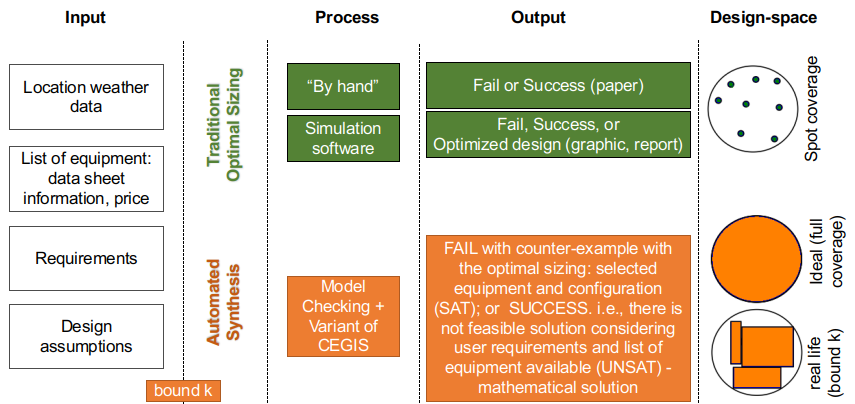
\includegraphics[width=1.0\textwidth]{optimalsizingprocess2}
\centering
\caption{Comparative of optimal sizing methods}
\label{fig:optimization}
\end{figure}
 
\subsection{Variant of CEGIS} 

In Figure~\ref{CEGISalt}, it is pictured a variant of CEGIS previously presented in Section ~\ref{sec:ProgramSynthesis}, Fig.~\ref{Counter-Example-Guided-Inductive-Synthesis}. This variant was created during this Thesis and it will be detailed in this Section.

\begin{figure}[h]
	\centering
	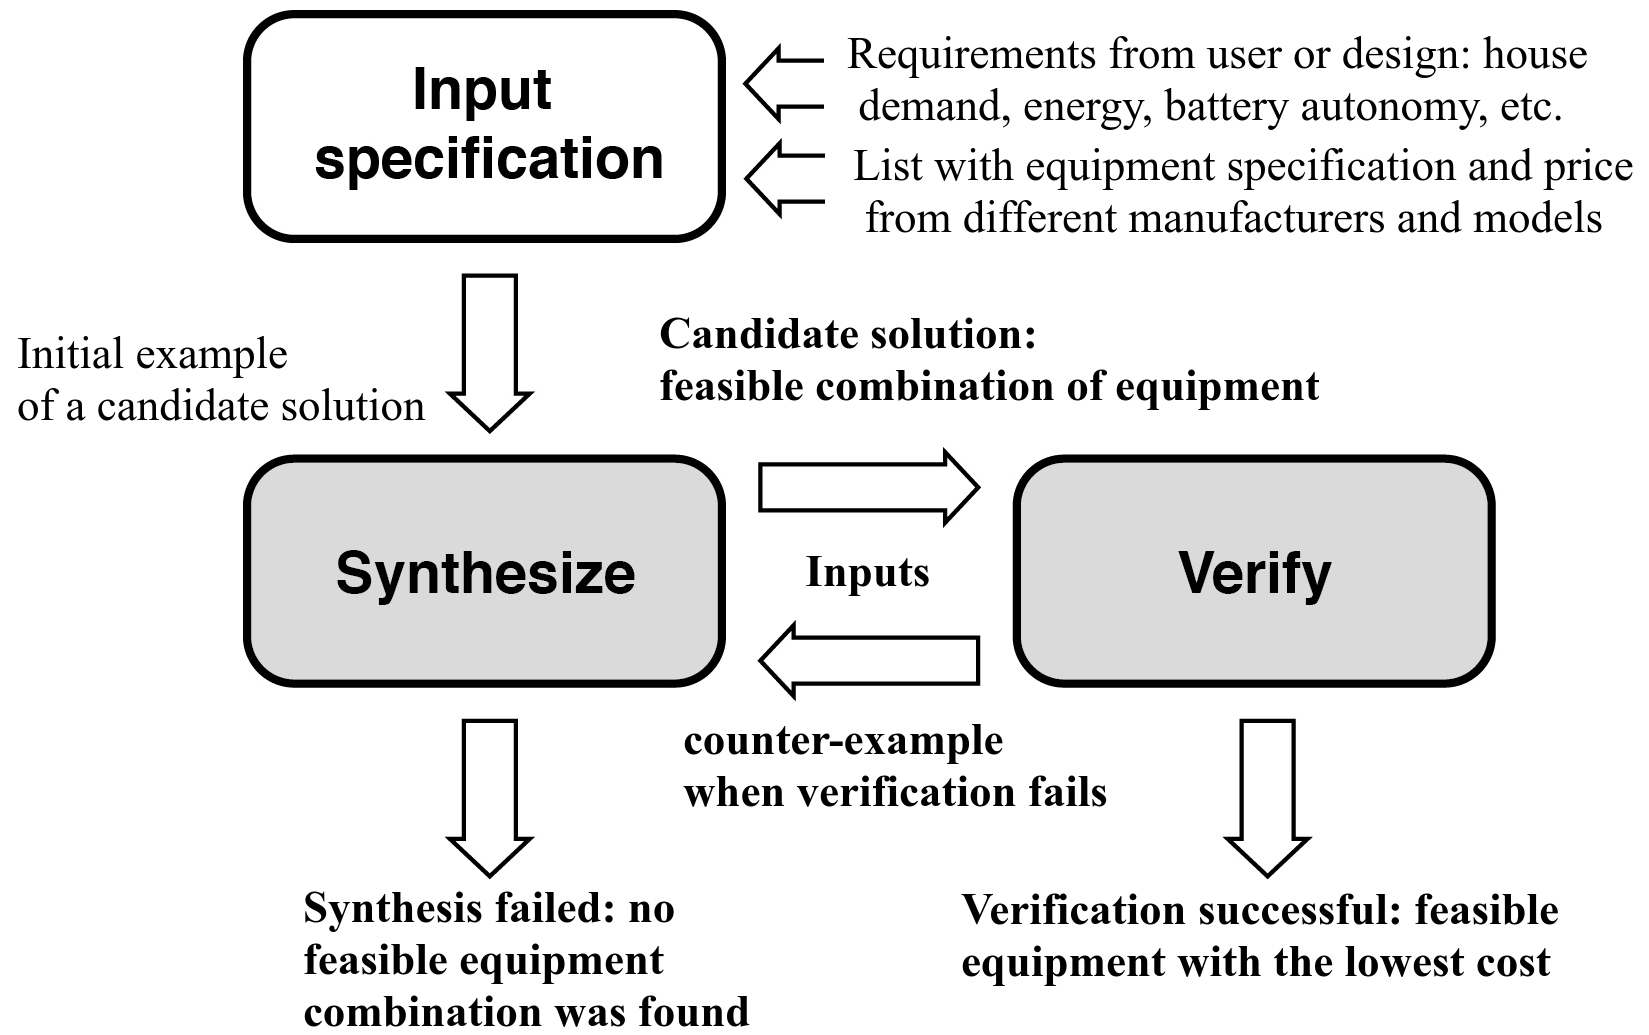
\includegraphics[width=0.75\columnwidth]{fig2_rev.jpg}
	\caption{CEGIS applied to PV system sizing.}
	\label{CEGISalt}
\end{figure}

Examples of specification used by the proposed method include solar insolation (site dependent), house power demand, house consumption energy, estimated load curve, AC voltage, and battery autonomy; we also provide a list of equipment specification and price from different manufacturers and models. Design assumptions are considered project specification as well. The assumptions regarding the optimal sizing are listed in Section~\ref{sec:OptAssumptions}.

There are four particular differences related to the traditional CEGIS described in Figure ~\ref{Counter-Example-Guided-Inductive-Synthesis} when compared to the variant CEGIS used in the proposed approach: 

\begin{itemize}
\item There exists no test vector and every candidate is generated during the run-time in the {\sc Synthesize} phase and sent to the {\sc Verify} phase; 
\item If the {\sc Verify} phase is unsuccessful, then a new candidate is generated by {\sc Synthesize} 
\item The lower bound of the {\sc Verify} phase is incremented to search for the lowest cost; 
\item As a result, there exists no refinement from the {\sc Verify} phase back to the {\sc Synthesize} phase, i.e., a new counterexample is not added to the {\sc input} set since a failure during the {\sc Verify} phase will only discard a given candidate that could be feasible in the next iteration with a new lower bound.
\end{itemize}

Program synthesis engines that implement the CEGIS approach~\cite{sketch} can automatically produce solutions for a large variety of specifications; here we have used symbolic software verifiers based on SMT solvers.


Algorithm~\ref{alg:opt-algorithm} describes our pseudo-code to synthesize stand-alone PV systems using symbolic model checking. It was adopted the analytical method of optimization, with LCC economical analysis and power reliability based on the critical period criteria.
%
 \begin{algorithm}
 \caption{Synthesis algorithm}
 \begin{algorithmic}[1]
 \renewcommand{\algorithmicrequire}{\textbf{Input:}}
 \renewcommand{\algorithmicensure}{\textbf{Output:}}
  \STATE Initialize variables \\
  \STATE Declare list of PV panels, controllers, batteries, and inverters data and cost \\
%  \STATE Declare list of controllers data and cost \\
%  \STATE Declare list of batteries data and cost \\
%  \STATE Declare list of inverters data and cost \\
  \STATE Declare the maximum possible cost $MaxCost$  \\
  \STATE Declare power demand, power peak, energy consumption \\
  \STATE Declare battery autonomy, deep of discharge, AC voltage \\
  \FOR {$HintCost=0$ to $MaxCost$}
 	\STATE Declare non-deterministic variable to select PV Panel from list \\
 	\STATE Declare non-deterministic variable to select Controller from list \\
 	\STATE Declare non-deterministic variable to select Battery from list \\
 	\STATE Declare non-deterministic variable to select Inverter from list \\ 	
 	\STATE Calculate $E_{corrected}, \, E_{p} $ \\
	\STATE Calculate $N_{TPmin}, \, N_{PSmin}, N_{PPmin} $ \\
 	\STATE Calculate $C_{bank}$ \\
	\STATE Calculate $N_{BS}min, \, N_{BP}min, \, N_{B}total$ \\
	\STATE Requirement enforced by \textbf{assume}$(V_{c})$ \\
 	\STATE Calculate $I_{sc,amb}$ \\
 	\STATE Calculate $I_{c,min}$ \\
 	\STATE Requirement enforced by \textbf{assume}$(I_{c} \wedge V_{in}DC \wedge V_{out}AC)$ \\
%	\STATE Requirement enforced by \textbf{assume}$(V_{in}DC \wedge V_{out}AC )$ \\
%	\STATE Requirement enforced by \textbf{assume}$(V_{out}AC)$ \\
	\STATE Requirement enforced by \textbf{assume}$(Demand \wedge P_{surge})$ \\
%	\STATE Requirement enforced by \textbf{assume}$(P_{surge})$ \\
	\STATE non-deterministic variables hold feasible equipment and cost  \\
	\STATE $F_{obj} \leftarrow  N_{TP}*Panel_{Cost} \, + \, N_{TB}*Battery_{Cost} \, + Controller_{Cost} \, + \, Inverter_{Cost} \, + \, Installation_{Cost} \, + \, batrep_{Cost} \, + \, PWO\&M_{Cost}$ \\
	\STATE Violation check with \textbf{assert}$(F_{obj} > HintCost)$ \\
  \ENDFOR
 \RETURN $(\,)$ 
 \end{algorithmic} 
 \label{alg:opt-algorithm}
 \end{algorithm}
%

Our synthesis algorithm will synthesize constant values; 
it starts with the input of manufacturers data and prices of PV panels, batteries, 
charge controllers and inverters (line $2$). After that, we define user requirements, i.e., 
house requirements and design definitions, from lines $4$ and $5$. 

The \textit{for}-loop started at line $6$ controls the lowest cost to the PV solution. 
In particular, it starts with cost $0$ and stops only when the algorithm finds a 
feasible solution in which the cost breaks the $assertion$ stated in line $22$; 
if that happens, then our algorithm has found an optimal solution, thereby stating 
that the {\sc Verify} phase reached a satisfiable condition (\textit{SAT}). 
The $MaxCost$ value at line $6$ is just a very high value put as a limit 
to the \textit{for}-loop, that never will be reached because the optimal solution will be found first.

Our synthesis algorithm uses non-deterministic variables to choose one specific constant 
from a given list of PV panels, controllers, batteries and inverters (lines $7$ to $10$). 
That procedure ensures that our synthesis engine checks all combinations of items 
from each equipment, and combine them to assemble a feasible (candidate) PV solution, 
which meets the user requirements.

Next, we use Eq.~\eqref{eq:Ecorrected}, Eq.~\eqref{eq:Ep}, Eq.~\eqref{eq:NTPmin}, 
Eq.~\eqref{eq:NPSmin}, Eq.~\eqref{eq:NPPmin}, Eq.~\eqref{eq:Cbank}, 
Eq.~\eqref{eq:Nbtotal}, Eq.~\eqref{eq:iscamb}, and Eq.~\eqref{eq:icmin} to calculate the sizing variables (lines $11$ to $17$). The directive \textit{assume} (lines $15$, $18$ and $19$) 
ensures the compatibility of the chosen items from the list of equipment: the {\sc Verify} phase 
uses only the item (among all the possible ones) that satisfies the statements of Lines $15$, $18$ and $19$. Line $15$ is specific to the charge controller voltage check. Line $18$ checks the inverter check $I_{c}$, charge controller DC input voltage $V_{in}DC$, and charge controller AC output voltage $V_{in}DC$ check. Line $19$ ensures the power demand and the surge power of inverter.
Therefore, our synthesis algorithm reaches line $20$ with one feasible solution, 
and the cost of that solution is calculated in $F_{obj}$ (line $21$). This cost is the equivalent of ~\ref{eq:LCC} described in Section ~\ref{sec:optcriteria}.

If our algorithm does not find a feasible solution among the item of equipment that 
were provided to our {\sc Synthesize} phase,  then the result is an unsatisfiable (\textit{UNSAT}), i.e., 
the program finishes and does not find a solution, which indicates that it 
was not possible to combine the items of each equipment in order to create a feasible solution. 

The main challenge for the {\sc Synthesize} phase is to find a feasible candidate 
solution regarding the constraints and user requirements. Related to our {\sc Verify} 
phase the challenge is to find the lowest acquisition cost from a list of equipment and 
components that is provided from the {\sc Synthesize} phase. 

Note that the process described here is completely automated and that a validation is performed 
by our {\sc Verify} phase to ensure that the approach is sound.

\subsection{Optimization Assumptions and Premises}
\label{sec:OptAssumptions}
%%%%%%%%%%%%%%%%%%%%%%%%%%%%%%%

Here some premise are presented and some adopted assumptions are explained for the optimal sizing method, regarding the automated synthesis and simulation software.

Regarding the line $2$ of Algorithm~\ref{alg:verification-algorithm}, 
a list of forty equipment from ten different manufacturers was provided 
to the synthesis engine in order to allow the choice of every item 
of PV sizing. Data sheet from each item was necessary to collect 
technical information. Moreover, the price of each item was obtained 
from available quotations in the market, and if the currency was not in US dollars, 
then it was used the exchange rate of the day to convert it to US dollars.

With respect to power reliability, this work will rely on the critical period solar 
energy method~\cite{Pinho} as described in Section~\ref{sec:sizing}. 
The usual way is to use loss of load probability (LOLP) or loss of power 
supply probability (LPSP). However, based on the fact that here we 
are neither considering site characteristics nor the load changes over time, 
which demands historical data, the reliability analysis will be developed only 
by the critical period method of PV sizing.

Regarding financial analysis:
\begin{itemize}
	\item LCC lifetime considered: $20$ years;
	\item Installation costs: includes delivery in the isolated community and installation costs itself, $5$\% of total cost~\cite{Agrener2013};
	\item Value of the discount rate or interest rate: $10$\%, which is a good rate considering financial investments in developing countries;
	\item Operation and maintenance annual costs: based on past PV projects of similar size in the Amazon region of Brazil, will be adopted the value of US\$ 289.64~\cite{Agrener2013}. This cost includes the battery replacement based on its lifetime ($4$ years for lead-acid batteries), plus inverters and controller replacement (every $10$ years). Therefore, it will be performed three battery bank and one inverter-controller replacements during the LCC analysis.
\end{itemize}

On the subject of PV system optimization technique, we will adopt here the intuitive method 
since the average value daily of solar irradiance is used in the mathematical model, 
without considering the battery's state of charge, or even the random nature 
of solar irradiation and meteorological conditions. Therefore, all the computational 
effort will be concentrated in our automated synthesis algorithm.

Regarding all case studies, it was defined that the minimum state of charge of batteries is $75$\% (with DOD maximum of $25$\%, which is common to lead-acid batteries), the voltage of the system is set in $24$ V DC (the most common as well, but the value can be adjusted to $12$ or $48$ V at the code), and the AC voltage from the inverter is $127$ V (Brazilian standard).

Related to off-the-shelf simulation tools only HOMER Pro and Hybrid2 perform off-grid system with battery backup analysis. Additionally, HOMER and RETScreen include economical analysis or even optimization-sensitive analysis. Therefore, in this study, HOMER Pro will be the simulation tool used to compare with our automated synthesis method.  Related to HOMER Pro:

\begin{itemize}
	\item HOMER Pro do not have the LCC cost in its reports. However, it has NPC and LCOE. Therefore NPC was used to obtain LCC in order to allow the comparative among tools;
	\item The optimization analysis of HOMER Pro allows to define a load curve and temperature according of data collected automatically from online databases. However, in order to allow a correct comparative, the curve load and the temperature were defined exactly the same as automated synthesis tools;
	\item Battery autonomy is not an parameter that the user can set when using HOMER Pro. The tool will always to meet the user requirement, i.e., the load curve during the $365$ days of the year;
	\item HOMER Pro do not have a explicit equipment called charge controller. It uses a controller resource that can perform in two different ways, according of the optimization choice or the user choice: load following or cycle charging~\cite{HOMER}. During the tests it was chosen the load following controller: it produces only enough power to meet the demand~\cite{HOMER};
	\item It was assumed the value of 5\% of capacity shortage that is equivalent to 95\% of availability of the PV system. By definition, availability is the percentage of time at which a power system is capable of meeting the load requirements~\cite{Khatib2014}. For critical loads, 99\% is considered acceptable. While in a ordinary house electrical load, 95\% is considered acceptable;
	\item It was assumed a string of two batteries in order to match the voltage of the system of $24$ V DC that was used for the automated synthesis tool;
	\item The premise adopted when using HOMER Pro it was that the user does not know the optimal solution, and that in order to obtain this solution is necessary to include (at the design phase of the tool) generic PV and batteries modules that HOMER Pro will search for the optimized power of each component. With that in mind, it was included a generic flat plate PV of $1$ kW and generic lead-acid batteries of $1$ kW as well (and with capacity of $83.4$ Ah according with HOMER Pro modeling). HOMER, during run-time, decides the size in kW of each module, based on feasibility and lower cost.
\end{itemize}

\section{Conclusion}

This Chapter showed in details how the automated verification method and the automated synthesis method, two state-of-art tools used in computer science, were adapted in order to be used in stand-alone solar PV systems to validate their behavior or the obtain the optimal project sizing. Moreover, is was possible to picture how the proposed methods are compared with the traditional ones used for the same purpose.

Detailed diagrams, flowcharts and algorithms with pseudo-code were presented with the aim to support the proposed work and to facilitate the understanding. And even more so, the assumptions adopted for the automated verification and simulation software were listed, because those assumptions have impact at the results there will be presented at the next two Chapters.

